%IMPORTANT!!!!!! remember to abilitate twoside, openright to print document.
\documentclass[12pt]{report}%, twoside, openright]{report}
\usepackage[english]{babel}
\usepackage[utf8]{inputenc}
\usepackage{amsmath}
\usepackage{graphicx}
\graphicspath{{diagrams/}}
\usepackage{listings}
\usepackage{dirtytalk}

\usepackage[backend=biber,
						bibstyle=ieee,
						sorting = nty,
						citestyle=numeric-verb]{biblatex}
\bibliography{bibliography.bib}
\begin{document}

\begin{titlepage}

\newcommand{\HRule}{\rule{\linewidth}{0.5mm}}

\center % Center everything on the page

\textsc{\LARGE Fachhochschule Dortmund}\\[1.5cm] % Name of your university/college
\textsc{\Large Master Thesis for M. Eng. in Embedded Systems for Mechatronics}\\[0.5cm] % Major heading such as course name

\HRule \\[0.4cm]
{ \bfseries Development of a real-time software architecture for AMiRo robot based on the operator controller-module}\\[0.4cm] % Title of your document
\HRule \\[1.5cm]

\begin{minipage}{0.4\textwidth}
\begin{flushleft} \large
\emph{Author:}\\
Hector Gerardo Munoz Hernandez
\end{flushleft}
\end{minipage}
~
\begin{minipage}{0.4\textwidth}
\begin{flushright} \large
\emph{Supervisors:} \\
Prof. Dr. Carsten Wolff

Uwe Jahn
\end{flushright}
\end{minipage}\\[2cm]

{\large \today}\\[2cm]

\vfill
\end{titlepage}
\pagenumbering{roman}
\tableofcontents

\begin{abstract}
This work covers most of the internal controller required functionality assigned to the DA\_AMiRo project. The architecture of the AMiRo is briefly discussed and it is then explained how the three boards of the AMiRo talk to each other. Some other sensors are explained, and the Communication Area Network module. All these functionalities are incorporated in the sensor data handler which is explained later. Every piece of code described in the present report is part of the DA\_AMiRo project and the reader can go to the gitlab repository and the Wiki page for more information. One of the purposes of the DA\_AMiRo project is to compare its functionality with the DAEbot project conducted by Uwe Jahn. The reader can read all about the DAEbot's internal controller in the previous student's work \cite{DAEBot_internal}. This work will finalize with a comparison on both systems.
\end{abstract}
\pagenumbering{arabic}

\chapter{Introduction}
\section{Real-time Operating Systems}
The necessity to meet deadlines in today's projects is every time more demanded. Most applications consist of different tasks that can be executed in parallel, have different priority, have different period repetition, and frequently use shared resources. Using a multi-threading approach, however,  can create a challenge in terms of performance, stability and time of implementation.

An operating system is a software component of a computer system that is responsible for the management and coordination of activities and the sharing of the resources of the computer \cite{mcgraw}. "A real-time operating system perform these tasks, but is designed to run applications with a very precise timing and a high degree of reliability. This can be especially important in measurement and automation systems where downtime is costly or a program delay could cause a safety hazard" \cite{rtos}.

In other words, a real-time operating system is an operational system that provides certain capability according to preset timing constraints \cite{whatisRTOS}. This is achieved through a scheduler that is designed to provide a deterministic execution pattern. And so, the RTOS are used in systems with critical timing requirements, when each task should be executed within a restricted time interval \cite{whatisRTOS}.

When it can be guaranteed that a task will never exceed a maximum amount of time in being completed, it can be said that the operative system is "hard real-time". If it can be guaranteed that a task will most of the time not exceed a maximum amount of time in being completed, it can be said that the operative system is "soft real-time". An airbag system is an example of a "hard real-time" system, where the task has to be guaranteed to execute always within a time limit. For a "soft real-time" example, a video streaming can be considered, where an occasional loss of data can be accepted because it does not compromise the whole functionality \cite{rtos}.

In the real-time operating systems the managing of the tasks is crucial. To this end, programmers have to decide which task is running at certain time and how other tasks can preempt the processing resources if their priorities are higher. In other words, manage the schedule of the tasks so that they meet with their deadlines.

Some of the main characteristics of a RTOS are the following:

\begin{itemize}
\item Determinism: An application timing can be guaranteed within a certain margin of error.
\item Soft and Hard Real-Time: The validity of data after meeting a deadline. In soft real-time the deadline is not that crucial but in hard real-time the meeting of the deadline is very important.
\item Jitter: Which is the amount of error in the timing of a task over subsequent iterations of a program or loop \cite{whatisRTOS}.
\end{itemize}

\section{Operator Controller Module}
The OCM was introduced by a group of Professors in the University of Paderborn. The concept aimed to structure and design a reconfigurable controller systems \cite{ocmAuto}. As mentioned before, there are three different levels in the OCM. The first one is the lowest level of the OCM also simply known as the Controller. This level interacts directly with the plant of the system, which means that the control signal is produced and measured here. It is also necessary that the software processing in this layer is quasi-continuous so that the measured values are processed in real-time conditions \cite{ocmAuto}.

The second layer is called the reflective operator. It is in this layer where the monitoring and the controlling routines are executed \cite{ocmAuto}. This layer does not have access to the actuators directly, because the Controller is already doing this. The expected result is that the Reflective Operator modifies the Controller, sometimes also changing between different pre-established Controller configurations. This level also requires a quasi-continuous operations like a continuous adaptation algorithm or a watchdog. This operator also has to operate under hard-time constraints because its relation with the Controller. In short, this layer serves as a interface between the Cognitive Operator and the Controller \cite{ocmAuto}.

The third layer is the Cognitive Operator. On this layer the system gathers information about itself and its environment to improve itself. This recollection of information can be done by applying various methods such as learning and model-based optimization among others. In other words, it is in this layer where the self-improvement takes place \cite{ocmAuto}.

This project focuses on the Controller and Reflective Operator of the AMiRo. The controller is the responsible for commanding the internal sensors of the STM32F32 boards inside AMiRo in real-time. This sensor information is then retrieved by the Reflective Operator with a demo application that will be explained later in this document inside section \ref{sect:example}.

\section{AMiRo}
The AMiRO project, which stand for Autonomous Mini Robot was started in the University of Bielefeld by Stefan Herbrechtsmeier and worked by Thomas Schöpping in collaboration with few others. The motivation for this project was to use small embedded systems in order to create a small robot that is easy to transport, usable on a table or the floor, appealing for young people, that is created with a modular approach is able to be extendable and customizable. With all of these aspects in mind, the result should be also a powerful tool for research and education \cite{AMiRo_ppt_v1}.

The preliminary work was conducted in the University of Paderborn in the form of the BeBot mini robot \cite{AMiRo_ppt_v1}. The intended architecture of both robots is a modular one, which means that it has more than one board functioning as a unity. In AMiRo's case, said architecture consisted on three boards, DiWheelDrive, Power Management, and Light Ring that will be discussed in the next chapter, and two main extension boards: the Cognition board and the Image Processing board. The former will be explained in section \ref{sub:cogn}, but the latter will not be discussed in this work, as it was not needed for the current reach of the project. If the reader is interested in the Image Processing board, he or she can refer to the project presentation given by Prof. Herbrechtsmeier \cite{AMiRo_ppt_v2}.

Physically AMiRo has a cylindrical shape with a diameter of 100mm. It is covered by a chassis that does not cover the DiWheelDrive board's bottom as this board has the proximity sensors pointing towards the ground. There are also two wheels with two separate motors directly connected to the DiWheelDrive board and two metal sliders for the robot stabilization in flat surfaces \cite{AMiRo_paper_modular}.

The chassis has three more openings for the following connections: USB serial that goes directly into the DiWheelDrive board, the power supply, and the charging pins. Additionally, when the Cognition board is attached, there are three more possibilities to physically interact with the robot: USB serial, USB dongle for wireless connection with the Linux OS, and a micro USB cable for connecting also with the Linux OS which is used in this board. The Cognition board will be later discussed in section \ref{sub:cogn}.

These characteristics make AMiRo a very compact and portable robot. Every board is designed to be modifiable, stackable and exchangeable with custom elements. All boards communicate with each other with the Controller Area Network protocol \cite{AMiRo_paper_modular}. This way every board can read any message from the CAN bus or write into it every time it is necessary.

\chapter{Architecture of AMiRo}
The AMiRo project was started in 2015 and ever since, the repository supporting the AMiRo project has had several updates \cite{AMiRo_Wiki}. It is worth mentioning that the version used as the basis for the present work was the version 1.0 stable. The AMiRo's repository consists of three basic folders: AMiRo bootloader, AMiRo Operating System, and ChibiOS.

Although this software architecture will be explained with more detail in section \ref{sec:soft}, it is worth mentioning that AMiRo's bootloader was used as it is in version 1.0 from the original repository in order to configure the computer for programming the AMiRo. The ChibiOS was also used as it is in version 1.0 from the repository \cite{AMiRo_Wiki}. The AMiRo Operating System was hugely modified to meet the requirements of the present work, which can be found under the current project's repository \textit{DA\_AMiRo} \cite{AMiRo_Git}.
%\footnote{AMiRo's original repository: https://openresearch.cit-ec.de/projects/amiro-os/wiki \cite{AMiRo_Wiki}}.

\section{Hardware Architecture of AMiRo}
As mentioned in the previous chapter, the AMiRo is equipped with three basic board modules and two extension boards. In this section each board will be briefly discussed with a special emphasis in the functionalities that are of interest for this work. For a more complete discussion about the boards or the AMiRo in general, the reader is invited to read the documentation referenced in this work, specially \cite{AMiRo_paper_verstaile, AMiRo_paper_modular, AMiRo_paper_applications, AMiRo_ppt_v1, AMiRo_ppt_v2} which can be found on the CITEC website or on the repository of this work on gitlab \cite{AMiRo_Git}.

The functionality of the sensors used in the project will be briefly explained in this chapter. For the explanation on how to read the output of the sensors that are sent via the Controller Area Network protocol, the reader is invited to jump directly into section \ref{sec:canconv} for reviewing the CAN convention used in the entire project and section \ref{sec:sensorout} for understanding each sensor's output.

\subsection{DiWheelDrive}
\label{sub:DWD}
The DiWheelDrive is the bottom board of the AMiRo. It is equipped with an ARM Cortex-M3 based STM32F103 MCU from STMicroelectronics \cite{AMiRo_paper_modular}. It is through the DiWheelDrive's UART interface that the AMiRo's three basic modules get programmed. Each board gets programmed at a time with help of the AMiRo bootloader which will be discussed in section \ref{sub:btl}.

This board has two motors of 1W DC. The purpose of having two motors was to be able to have a differential kinematic to allow flexible movements \cite{AMiRo_paper_modular}. Among other sensors and actuators, the ones that are in this board and are being used in this work are: three axis gyroscope, accelerometer, and magnetometer, floor proximity sensors, the two motors, and optical motor encoders. The functionality and some specifications of the above mentioned sensors and actuators will be discussed in the next subsections.

As mentioned before, the DiWheelDrive board has a Cortex-M3 MCU for calculating such things as motion control, odometry, and dead reckoning algorithms at high sampling rates \cite{AMiRo_paper_modular}. This board can be accessed by the other boards via the Controller Area Network protocol or via USB UART interface directly with the user. It is important to mention that every board has also a USB UART interface to communicate directly with the user but they are covered by the chassis except for the DiWheelDrive board \cite{AMiRo_paper_modular}.

\subsubsection{Gyroscope}
The gyroscope is a sensor that measures rotational motion. The units of the resulting measurement are revolutions per second or degrees per second. As a quick example, in a balancing robot a gyroscope can be used to measure how much the robot has rotated from the desired position and this information can be sent to an actuator to make corrections in order to reach the desired angle \cite{gyrostheory}. A gyroscope normally consists of a mass that moves with constant angular momentum, so when the gyroscope is tilted the axis of rotation of said mass reacts to the applied rotational movements making the axis of rotation tilt. This tilting leads to a displacement of the capacitance fingers inside the sensor which changes the capacitance. Finally when compared to a reference capacitance level, the angular velocity can be determined \cite{AMiRo_ppt_v1}.

The gyroscope used in the DiWheelDrive board is the l3g4200d from STMicroelectronics. This sensor communicates via SPI with the processor. This sensor is configured to have a resolution of +-500 dps in accordance with the user's manual \cite{gyroscopepart} and it is possible to obtain the output in degrees per second, micro degrees per second, revolutions per second, and micro revolutions per second with the actual code. The actual units are degrees per second but the user can easily change the output selecting a different function from \textit{updateSensorVal()} function inside DiWheelDrive.cpp. For a more clear explanation on the code structure, see section \ref{AMiRo_OS}. The sensor communicates with the processor via SPI communication.

\subsubsection{Accelerometer}
The accelerometer is a sensor that measures the acceleration of an object. The units of the resulting measurement are meters per squared second or in g forces, where g as a unit equals $9.81 m/s^2$ \cite{accelerometertheory}. It is typically a system composed by a mass, a spring, and a damper. The mass moves according to the applied acceleration and changes the resulting capacitance that can be sent as an output for further reading and processing \cite{AMiRo_ppt_v1}.

The accelerometer used in the DiWheelDrive board is the lis331dlh from STMicroelectronics. This sensor is configured be scaled with a +/-8g factor in accordance with the user's manual \cite{accelerometerpart}. The output is in g units and the sensor is being communicated via SPI with the processor.

\subsubsection{Magnetometer}
The magnetometer is a sensor that measures the magnetic field for all three physical axes \cite{magnetometertheory}. This sensor works thanks to three principles. The first one is called the Anisotropic magneto resistance effect discovered in 1857 by William Thomson, in which an external magnetic field can make the sensor change the electrical resistance of a ferromagnetic material. The electrical resistance will be at a maximum value when the direction of the electrical current is parallel to said magnetic field \cite{AMiRo_ppt_v1}.

The second principle is called Fluxgate and it is a way of calculate the vectorial measurement of a magnetic field invented by Friedrich Förster in 1937. The method starts with two cores wrapped by two coils of wire. There should be an electrical current driving the core through cycles of magnetic saturation. The resulting electrical current of the second coil will depend on the external magnetic field \cite{AMiRo_ppt_v1}.

The last principle is called the Hall effect discovered in 1897 by Edwin Hall. In this principle can be visible when an electric current flows through a conductor in a magnetic field, the magnetic field will exert a transverse force on the moving charge carriers which tends to push them to one side of the conductor. The result is a voltage difference between both sides of the conductor \cite{halleffect}.

The magnetometer used in the DiWheelDrive board is the hmc5883l from STMicroelectronics. This sensor is configured to have a field resolution of +/-5Gauss according to the user's manual \cite{magnetometerpart} and the current output is set to be in Gauss units. The sensor is being communicated via I2C protocol with the processor.

\subsubsection{Floor Proximity Sensor}
\label{sec:AMS}
The floor proximity sensor used is the "Fully Integrated Proximity and Ambient Light Sensor With Infrared Emitter", part vcnl4020 of Vishay \cite{proxsensor}. Four of these sensors are in the bottom of the AMiRo, programmed as light sensors, while other eight of these sensors are being used as proximity sensors and ambient light detectors coordinated by the Power Management board, see section \ref{PWB} for more information.

The ambient light sensor measures the intensity of light and its is measured in luminance. In order to do this the sensor usually consists of a photoresistor or a photo-sensitive material, outputting a resistance that can be measured and compared to a default value to estimate the luminance \cite{amstheory}.

The goal of providing AMiRo with these sensors attached to its bottom is to detect changes in the color of the floor. An example application can be for the AMiRo to follow a line or path painted on the ground, by making the robot recognize when it is over one color and when it is not.

\subsubsection{Motors}
As previously described in section \ref{sub:DWD}, the AMiRo has two DC motors of 1W each to offer a differential kinematic and to allow agile movements \cite{AMiRo_paper_modular}. These motors are connected to the DiWheelDrive board which means that this board controls the velocity of the motors and also knows the actual velocity of the motors.

The velocity of the motors can be set anytime from the Cognition board and the actual velocity of the AMiRo is one of the sensor values that can be asked from AMiRo's internal controller. The user can set and view the velocity in $\mu m/s$ or in $\mu rad/s$.

\subsubsection{Encoder}
AMiRo has optical encoders as well, that allow the user to know how much the motors have turned from a certain checkpoint. This data can be used to know how far the AMiRo has moved from a certain point. This sensor returns the $x$ coordinate in $\mu m$, the $y$ coordinate in $\mu m$, and the orientation of the wheels in $\mu rad$

\subsection{Power Management}
\label{PWB}
The Power Management board is the central basic module of AMiRo. This board is responsible for the power supply and elementary behavior of the system. This is why it has the most powerful microcontroller. This board has an ARM Cortex-M4 based STM32F405 from STMicroelectronics. The characteristics from this microcontroller were needed to ensure a fast reaction times on critical system events and still provide enough headroom to additionally perform basic behaviors like obstacle avoidance, or homing \cite{AMiRo_paper_modular}.

There are two lithium-ion batteries connected to the Power Management board that power the whole system, and there are also some sensors on this board. Among the sensors that this board has, the ones that are being used by this project are: eight proximity sensors that act as proximity sensors and also as ambient light sensors, sensors for knowing if the charging cable is connected, the remaining battery charge or the time for a complete battery charge, the time for this both events to be completed, and the actual current consumption  \cite{AMiRo_paper_modular}.

\subsubsection{Power Status}
For the tracking of the power status, AMiRo is equipped with a bq27500 Impedance Track from Texas Instruments that allows the robot to obtain information such as remaining battery capacity, state-of-charge, run-time to empty, battery voltage, and temperature \cite{impedancepart}.

\subsubsection{Proximity Ring}
As seen in section \ref{sec:AMS}, the eight vcnl4020 sensors in connected to the Power Management board are functioning as ambient light sensors and also as proximity sensors. For this last functionality, the sensor has a built-in infrared emitter and photo-pin-diode, having a maximum relying measurement of 200mm \cite{proxsensor}. These sensors are connected in a ring-fashion way so that the AMiRo has eight sensors throughout its entire circumference, making it able to detect obstacles in all horizontal directions. The units of the output are also in mm.

\subsection{Light Ring}
The Light Ring board is the top-most board in the AMiRo. This board has a STMicroelectronics ARM Cortex-M3 based STM32F103 MCU. It contains eight RGB LEDs arranged in a circular way corresponding to the Proximity Ring discussed in last section. These LEDs can be set from the Cognition board, setting each color of the RGB channels \cite{AMiRo_paper_modular}.

\subsection{Cognition Board}
\label{sub:cogn}
This board was thought as an extension board which is no longer from the basic set of boards that make the AMiRo. The Cognition board in this project is being used as the Reflective Operator according to the OCM model. It provides all of the high-level tasks, gathering and coordinating the information generated in the three basic boards also known as the internal controller \cite{AMiRo_paper_modular}.

The most important feature of this board is the attached Gumstix Overo Computer-on-Module. In the current setup, the Overo TidalSTORM COM is being used, which combines an ARM Cortex-A8 based DaVinci DM3730 SoC from Texas Instruments \cite{AMiRo_paper_modular}. This board has the same serial programming port as on the three basic boards. It also has a Type A, a micro-AB, and an internal pin header USB interfaces \cite{AMiRo_paper_modular}.

The operating system running on the Overo COM is based on the Linux Yocto reference distribution Poky \cite{poky}, and the way it communicates with the three basic boards is through CAN, using a simple SocketCAN software-wrapper that is offered by this distribution \cite{AMiRo_paper_modular}.

\section{Software Architecture of AMiRo}
\label{sec:soft}
As it has been discussed in previous sections, the AMiRo project was started back in 2015 and it is still being maintained. The version 1.0 of the repository is the one being used for this project \cite{AMiRo_Git}.

\subsection{AMiRo bootloader}
\label{sub:btl}
The open-source bootloader for MCUs is the bootstrap for the three basic boards of the AMiRo. The AMiRo's bootloader is the responsible of configuring and setting up the computer for working with the AMiRo. The set-up that is provided in the bootloader is more than enough to successfully start working on the Operating System of AMiRo and programming it \cite{btl}.

As said before, the DiWheelDrive is the only module of which the programming port can be accessed by the user. This is why new software is applied to the two other basic boards by remote flashing via OpenBLT. Using CAN communication the new binary is forwarded by the DiWheelDrive board so that the target board receives the data and stores it in its flash memory \cite{AMiRo_paper_modular}.

\subsection{AMiRo real-time operating system kernel}
For the real-time operating system the open-source ChibiOS was chosen. This project aims at creating a portable, light weight, and fast real-time operating system for embedded applications \cite{chibioshp}. ChibiOS not only provides low-level drivers for all interfaces of the most common microcontrollers, it also gives an unified hardware abstraction layer, priority based preemptive scheduling, and high-performance event and message passing systems. ChibiOS can be configured statically and dynamically to exactly fit the application in order to maximize efficiency and performance \cite{AMiRo_paper_modular}.

\subsubsection{ChibiOS}
Some of the main characteristics from ChibiOS are:

\begin{itemize}
\item System time: ChibiOS has a 16 or 32 bits system time counter.
\item Real tick-less mode: There is no periodic system tick for optimal power management.
\item IRQ Management: ISRs abstraction.
\item Preemption: Fully preemptive scheduling.
\item Round robin scheduling: Round robin scheduling for threads at equal priority.
\item Messages: Inter-thread synchronous messages.
\item Mailboxes: Message queues.
\item Counter semaphores: Semaphores with boolean state.
\item Binary semaphores: Semaphores with boolean state.
\item Mutexes: Mutexes implementing the priority inheritance algorithm.
\item Events: Events, event flags, event sources.
\item Dynamic services: Dynamic threading.
\end{itemize}
Note: All the above mentioned characteristics can be found and further explained in the ChibiOS homepage. \cite{chibioshp}

A project containing ChibiOS consists on the Operating System source files, few configuration files and a HAL file for the peripherals handling.

\subsection{AMiRo Operating System}
\label{AMiRo_OS}
AMiRo's Operating System or board specific abstraction layer from the original repository \cite{AMiRo_Wiki} includes two basic applications, the first one is a rudimentary command shell and the second one a hardware test. The first one is already integrated in ChibiOS and it is extended by module specific commands \cite{AMiRo_paper_modular}.

The structure of the AMiRo Operating System, including the files that are being used with the current project can be visualized in figure \ref{fig:OS}. The entire project is written in C++ language, with some inclusions of C code. In this figure, it can be seen that inside \textit{AMiRo\_OS} there is the \textit{components} folder which contains the shared codes that the three boards are using. The other part of the structure worth mentioning now is the \textit{devices} folder in which the three boards have their own set of files, always maintaining the same structure among them.

\begin{figure}[ht]
	\centering
	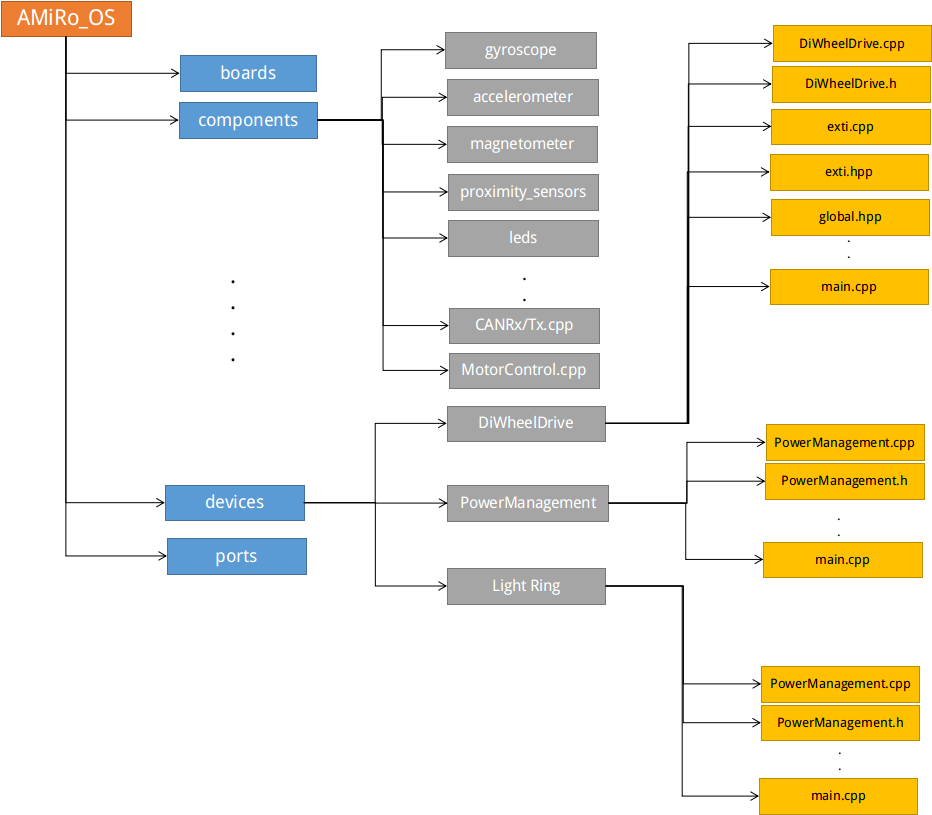
\includegraphics[width=\textwidth]{AMiRo_OS}
    \caption{AMiRo\_OS breakdown structure}
    \label{fig:OS}
\end{figure}

%Quizás algo más a cerca de AMiRo (apps, applicaciones pensadas, demos....)

\subsection{Overall structure}
From the past sections the hardware and software structure of the AMiRo was mentioned and briefly discussed. From this point forward the structure and functionality of the DA\_AMiRo project will be discussed as it is the central point of the master thesis. As a friendly reminder, the reader can obtain the source codes made for the DA\_AMiRo project from the repository \cite{AMiRo_Git}.

Taking into consideration once again figure \ref{fig:OS}, the 
%talk about the DA_AMiRo structure, which ones where modified, which ones where maintained as they were, and talk about the classes heritage. (class diagram)

\chapter{Controller Area Network}

This chapter explains how to receive and transmit CAN frames in the AMiRo. The functionality of the CAN module had to be merged with the current ControllerAreaNetworkRx.cpp and ControllerAreaNetworkTx.cpp of the existing repository of AMiRo \cite{AMiRo_Wiki}. The ControllerAreaNetwork.h however, is the same that the DAEbot project is using. The reason behind sharing the ControllerAreaNetwork.h among projects is to be able to use a single Relfective Operator for both systems AMiRo and DAEbot so it is easier to compare functionalities.

\section{Convention used for sending and receiving frames}
\label{sec:canconv}

The format of the CAN frames was done accordingly with the pre-established convention for the DAEbot project \cite{DAEbot_Wiki}. See figure \ref{fig:can}

\begin{figure}[ht]
	\centering
	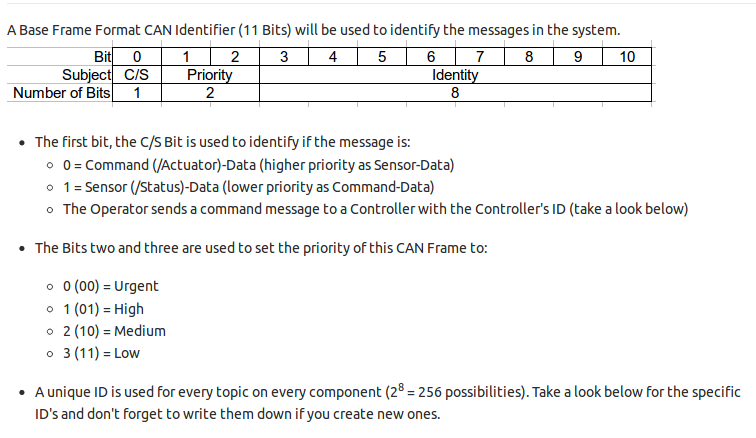
\includegraphics[width=\textwidth]{can_structure}
    \caption{Pre-established CAN frame format}
    \label{fig:can}
\end{figure}

For the transmission of a CAN frame, the id is coded according to figure \ref{fig:can} and when a CAN frame is received, the id is decoded into the same structure. The CAN frame pre-established structure can be seen in snip of code \ref{CAN:frame}, which can be compared with the figure \ref{fig:can}.

\begin{minipage}{\linewidth}
\begin{lstlisting}[caption = CAN frame, label = CAN:frame, language = C, captionpos = b]
typedef struct can_frame_types {
    priority_can_id_t priority_id;
    c_s_bit_can_id_t c_s_bit_id;
    topic_can_id_t topic_id;
    uint8_t dlc;
    union{
        uint8_t     data8[8];
        uint16_t    data16[4];
        uint32_t    data32[2];
    };
} can_frame_types_t;
\end{lstlisting}
\end{minipage}

In order to send a CAN frame, can\_transmit\_data\_frame\_pd(...) can be called. When sending a CAN frame, the id is set to be in standard mode. The CAN frame that is sent consists of three main parts: id, DLC, and the data. The id is therefore set with the can\_code\_identifier\_pd(...) function before actually calling the transmit function. This function combines the c\_s bit with the priority bit and then combines that value to the topic ID. The CAN frame is sent with the function HAL\_CAN\_Transmit(...).

On the CAN reception side, the status of the reception is assigned when calling to the can\_receive\_data\_frame\_pd(...) function. The status of the CAN reception can be successful, timeout, or error. Then the id of the CAN frame gets decoded with the function can\_decode\_identifier\_pd(...) and the data frames are passed into a global structure like in snip of code \ref{CAN:frame}

Note that can\_code\_identifier\_pd(...) and can\_decode\_identifier\_pd(...) are functions that were already implemented beforehand, for this project it was necessary to adjust both functions to operate with the current hardware platform.

\section{Interpreting outputs of the sensors}
\label{sec:sensorout}
%explicar cómo interpretar valores de sensores.

\chapter{Sensor data handler}
\section{Overall functionality}

\section{Implementing modes}

\section{Real-time implementation}
%al final decir que funciona ya independientemente como un sólo internal controller.

\chapter{MuRoX}
\section{Compiling for MuRoX}

\section{Example application}
\label{sect:example}

\chapter{Matlab}
\section{Compiling from Simulink for MuRoX}

\chapter{Results}
\section{AMiRo vs. DAEbot}

\section{Outlook}

\iffalse
The DAEbot which stands for Distributed Architectures Evaluation Robot, is part of the Ph.D. student Uwe Jahn's project. The DAEbot by itself has the objective of testing different approaches for distributed software and hardware architectures \cite{DAEbot_Wiki}. The robot was designed with the goal of having a modular platform and therefore, the hardware is also easily interchangeable for adapting to different software distributions or different applications\cite{DAEbot_Wiki}.

The DAEbot works according to a OCM \cite{ocmAuto} software architecture where there are three basic controllers: Internal Controller, Reflective Operator, and Cognitive Operator. In order to have a more precise overview of how these three controllers work in the DAEbot, figure \ref{fig:ocm} is explained by a direct quote from the Wiki:

\say{Refering to figure \ref{fig:ocm}, the Controllers (red) are used to connect all sensors and actuators. The Controllers need to be configured and programmed once, so the software on the controllers is mostly fixed and does not need to be flexible. The Reflective Operator(s) (yellow) control the Controllers. The Reflective Operator's software is the adaptable part of the distributed system - it changes from application to application. These Operator Controller Module(s) are located on the robot itself and let it act autonomously. The Cognitive Operator is hosted on a server and is used to optimize, program and interact with the user. The Cognitive Operator is connected via a wireless connection and can (only) interact with the Reflective Operator(s).}\cite{DAEbot_Wiki}.

\begin{figure}[h!t]
	\centering
	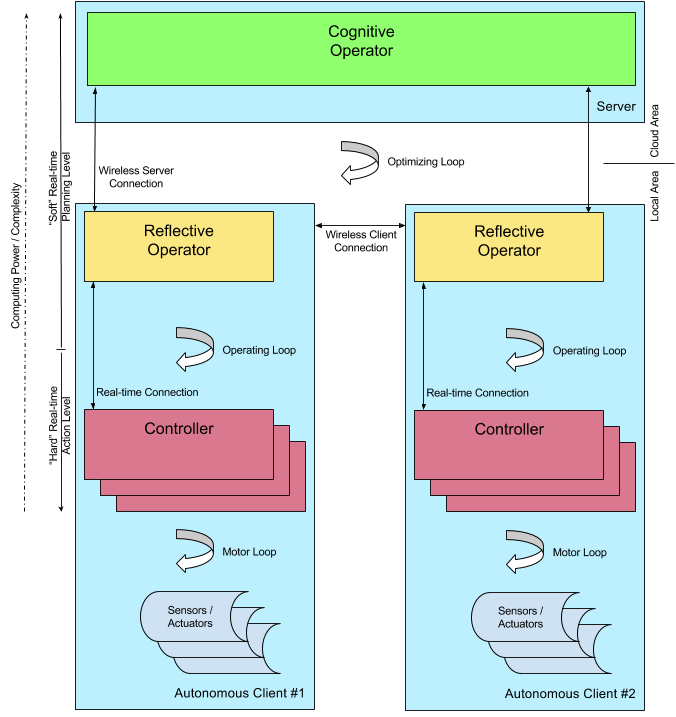
\includegraphics[width=\textwidth]{ocm}
    \caption{OCM software arquitecture for the DAEbot\cite{DAEbot_Wiki}.}
    \label{fig:ocm}
\end{figure}
\clearpage




\chapter{Hardware Drivers}
The used hardware was a STM32F3DISCOVERY board which among other features, has:
\begin{itemize}
\item Gyroscope, available through a SPI interface (part no. L3GD20).
\item Accelerometer, available through a SPI or I2C interface (part no. LSM303DLHC).
\item Magnetometer, which is a part of the Accelerometer part (part no. LSM303DLHC).
\item CAN module, which outputs a CANtx and CANrx that can be then connected to an external CAN module that transforms the signal into CAN high/low.
\item GPIO pins that were used in this project as LEDS for debugging, and also for the ultrasonic sensors. The details about the ultrasonic sensors can be obtained in section \ref{sect:ultras}.
\end{itemize}

\section{Internal STM32F3 sensors}
This section covers the configuration used and needed to successfully communicate with the peripherals employed in this project.

The corresponding codes for this section can be found in the following project paths:
\begin{itemize}
\item \textit{DAEbot/Peripheral-Drivers/DAEbot-PD/STM32F3Drivers/InternalSensors}, where the files for the internal sensors which contains configuration and handling of gyroscope, accelerometer, and magnetometer can be found.
\item \textit{DAEbot/Peripheral-Drivers/DAEbot-PD/STM32F3Drivers/UltrasonicSensors}, where the files for the configuration and handling of the ultrasonic sensors can be found.
\item \textit{DAEbot/Peripheral-Drivers/DAEbot-PD/ControllerAreaNetwork}, where the files for the configuration and handling of the CAN communication can be found under the macro \#ifdef STM32F3\_DAEbot.
\item \textit{DAEbot/Devices/Internal\_Robot\_CTRL}, where the main implementation of the project is being done. Here is the code that uses the configuration files mentioned above and handles the FreeRTOS task scheduling.
\end{itemize}

The gyroscope, accelerometer, and magnetometer are communicated via SPI and I2C. The configuration of them has to be as follows:

Configuration for the SPI:
\begin{itemize}
\item Mode: master.
\item Direction: 2 lines.
\item Clock polarity: low.
\item Baud rate prescaler: 16
\item Polynomial for CRC calculation: 7
\end{itemize}

Configuration for the I2C:
\begin{itemize}
\item Timing register value = 0x00902025.
\item Own address: 0.
\item Addressing mode: 7 bit.
\end{itemize}

\subsection{Gyroscope}
The gyroscope part is called L3GD20\cite{gyroscopepart}, this sensor is communicated with the processor via SPI. To initiate the sensor it is necessary to enable the desired axis writing a 0xCF to the 0x20 address registry (CTRL\_REG1) which corresponds to enabling all the axis and setting a 760Hz frequency.

In order to obtain data from the gyroscope and have it back in the processor, the address 0x27 is transmitted to the gyroscope and the gyroscope will output the data from the three axis in a 64-bit per axis fashion. To accomplish this, the gyroscope has a low part of 32 bits and a high part of 64 bits for each axis in the following manner:

\begin{itemize}
\item Coordinate "x\_low" 0x28
\item Coordinate "x\_high" 0x29
\item Coordinate "y\_low" 0x2A
\item Coordinate "y\_high" 0x2B
\item Coordinate "z\_low" 0x2C
\item Coordinate "z\_high" 0x2D
\end{itemize}
To normalize the output the following conversion was used:

\begin{equation} \label{eq:gyroscope}
	result = \frac{value * mdpsperdigit}{1000}
\end{equation}

Where the value is the raw number received from the peripheral and mdps per digit is a fixed value of 8.75 which calibrates the gyroscope and outputs a value in revolutions per second.

\subsection{Accelerometer}
The accelerometer part is called LSM303DLHC\cite{accelerometerpart}, this sensor is communicated with the processor via I2C. To initiate the sensor it is necessary to enable the desired axis writing to the 0x20 address registry (CTRL\_REG1\_A) a 0x57 which corresponds to enabling all the axis and setting  a low-power mode of 100Hz.

In order to obtain data from the accelerometer and have it back in the processor, the address 0x27 is transmitted to the accelerometer which has a slave address of 0011001. Afterwards the accelerometer will output the data from the three axis in a 64-bit per axis fashion. To accomplish this, the accelerometer has a low part of 32 bits and a high part of 64 bits for each axis in the following manner:

\begin{itemize}
\item Coordinate "x\_low" 0x28
\item Coordinate "x\_high" 0x29
\item Coordinate "y\_low" 0x2A
\item Coordinate "y\_high" 0x2B
\item Coordinate "z\_low" 0x2C
\item Coordinate "z\_high" 0x2D
\end{itemize}

To normalize the output the following conversion was used:

\begin{equation} \label{eq:accelerometer}
	result = \frac{value * 4 * g}{65535}
\end{equation}

Where the value is the raw number received from the peripheral and g is the acceleration of gravity $9.81 \frac{m}{s^2}$. The resulting value will be also in $\frac{m}{s^2}$ units.

\subsection{Magnetometer}
The magnetometer part is the same as the accelerometer: LSM303DLHC\cite{accelerometerpart}, this sensor is communicated with the processor also via I2C. To initiate the sensor it is necessary to enable the desired axis writing to the 0x00 address registry (CTRL\_REG1\_M) a 0x3C which corresponds to configure the minimum data output rate to 220Hz. Also, the address 0x02 is written with a 0x00 to specify that the data conversion mode must be continuous.

In order to obtain data from the magnetometer and have it back in the processor, the slave address of the magnetometer 0011110x is sent via I2C to the peripheral. The x is a write/read bit so for the purpose of receiving the data from the magnetometer a 0x3c has to be sent. Afterwards the magnetometer will output the data from the three axis in a 64-bit per axis fashion. To accomplish this, the magnetometer has a low part of 32 bits and a high part of 64 bits for each axis in the following manner:

\begin{itemize}
\item Coordinate "x\_low" 0x03
\item Coordinate "x\_high" 0x04
\item Coordinate "y\_low" 0x05
\item Coordinate "y\_high" 0x06
\item Coordinate "z\_low" 0x07
\item Coordinate "z\_high" 0x08
\end{itemize}

To normalize the output the following conversion was used:

\begin{equation} \label{eq:magnetometer}
	result = value * 1.22
\end{equation}

Where the value is the raw number received from the peripheral and mdps per digit is a fixed value of 8.75 which calibrates the gyroscope, outputing a value in gauss units.

\section{Ultrasonic sensors}
\label{sect:ultras}
The four ultrasonic sensors are connected via GPIO. Each ultrasonic sensor has four pins: 5V input, ground, trigger pin, and echo pin. The final layout of the pins can be seen in table \ref{tab:ultras}.
\begin{table}[h!]
\centering
\begin{tabular}{l|c|c}
Ultrasonic sensor & Trigger pin & Echo pin \\\hline
1st	&	PC2		&	PC3		\\
2nd	&	PD10	&	PD11	\\
3rd	&	PB10	&	PB11	\\
4th	&	PB2		&	PE7
\end{tabular}
\caption{\label{tab:ultras}Ultrasonic sensors mapping to STM32F3DISCOVERY}
\end{table}

For each ultrasonic sensor the reading process is the following:
\begin{enumerate}
\item Write trigger pin a '0'.
\item wait for 2 $\mu s$
\item Write trigger pin a '1'.
\item wait for 10 $\mu s$
\item Write trigger pin a '0'.
\item Wait for a response in the echo pin.
\item Count time the echo pin is being written with '1'.
\item Normalize the output.
\end{enumerate}

To normalize the output the following conversion was used:

\begin{equation} \label{eq:ultras}
	distance = \frac{time\_in\_'1'}{58-20}
\end{equation}
Where the distance variable is the distance in cm from the ultrasonic sensor to an object.

Note: for the timing tasks, the vtaskDelay() of FreeRTOS function was used, taking into consideration that the clock frequency is set to 1MHz. This is why the function readUltrasonic() of the ultrasonic.c code can only be called from within a FreeRTOS task.

\section{CAN module}
The STM32F3DISCOVERY has a Controller Area Module interface in digital output. The assigned pins in the board are assigned as follows:

\begin{table}[h]
\center
\begin{tabular}{c|c}
CAN interface & Pin \\\hline
CANrx\_0	&	PA11		\\
CANtx\_0	&	PA12		\\
CANrx\_1	&	PB8			\\
CANtx\_1	&	PB9			\\
CANrx\_2	&	PD0			\\
CANtx\_2	&	PD1
\end{tabular}
\caption{\label{tab:pinCAN}CAN interfaces mapping to STM32F3DISCOVERY}
\end{table}

The chosen pins for the CAN module in this project were PD0 and PD1 as these are the pins which are hard-wired in the expansion board the STM32F3DISCOVERY board is being mounted. In order to use the CAN module, said GPIO pins have to be configured in the following fashion:
\begin{itemize}
\item Alternate function push pull mode.
\item Nor pull-up or pull-down.
\item High frequency mode.
\item CAN alternate function which according to the HAL drivers, is the value 0x07.
\end{itemize}

With the pins initialized, the CAN module was configured as follows.

\begin{itemize}
\item Normal mode.
\item Maximum time quanta = 1.
\item time quanta in bit segment 1 = 2.
\item time quanta in bit segment 2 = 3.
\item Prescaler of 8.
\item CAN filter in ID mask mode.
\item CAN filter scale of 32 bit.
\end{itemize}

The baud rate requirement of the CAN project was set to 500kHz. This frequency was achieved with the following equation:

\begin{equation} \label{eq:baudrate1}
	500kHz= \frac{24MHz}{(B1+B2+SW)*prescaler}
\end{equation}

Where the 24MHz is the clock frequency of the STM32F3 for the CAN module, the B1 and B2 are the time quanta bit segment one and two accordingly. Finally, the SW represents the maximum time quanta.

In order to accomplish this frequency a process of trial and error was conducted, given that the equation \ref{eq:baudrate1} has four unknown values. Firstly a 32 prescaler was set and the time quantas were made one variable which as so: $B1 + B2 + SW = TQ$. This resulted into the next equation:

\begin{equation} \label{eq:baudrate2}
	500kHz= \frac{24MHz}{(TQ)*8}
\end{equation}

And so,

\begin{equation} \label{eq:baudrate3}
	TQ = 6
\end{equation}

With this result the values of the time quantas can be assigned, taking into consideration that a value of 0 in any of this variables did not work as expected. So taking into consideration equation \ref{eq:baudrate4} the assignments were conducted as follows: $SW=1$ $B1=2$ $B2=3$.

\begin{equation} \label{eq:baudrate4}
	6 = B1+B2+SW
\end{equation}

And so the initialization of the peripherals has been exposed, also the functionality of the internal sensors have been explained. The functionality of the CAN interface, however, will be explained in the next chapter.

\chapter{CAN interface}
This chapter explains how to receive and transmit CAN frames in the STM32F3DISCOVERY board. The functionality of the CAN module of the STM32 board had to be merged with the current ControllerAreaNetwork.c and .h that other instances of the DAEbot project area already using.

It is important to take into consideration that the format of the CAN frames was done accordingly with the pre-established DAEbot project. See figure \ref{fig:can}

\begin{figure}[ht]
	\centering
	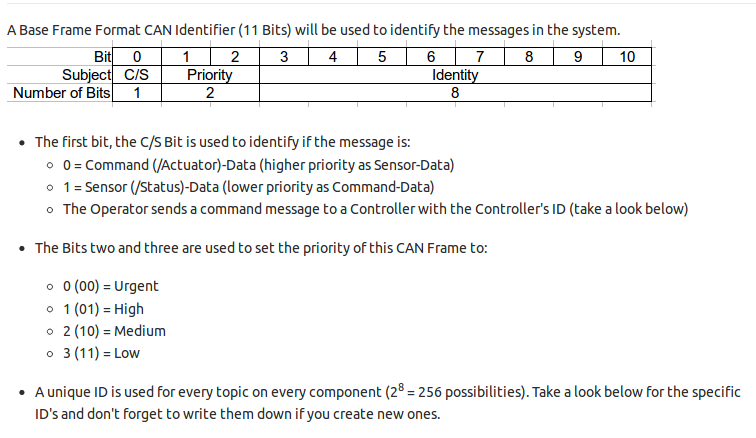
\includegraphics[width=\textwidth]{can_structure}
    \caption{Pre-established CAN frame format}
    \label{fig:can}
\end{figure}

\section{Functionality of Controller AreaNetwork.c /.h}

Upon the transmission of a CAN frame, the id is coded according to figure \ref{fig:can} and when a CAN frame is received, the id is decoded into the same structure. The CAN frame pre-established structure can be seen in snip of code \ref{CAN:frame}, which can be compared with the figure \ref{fig:can}.

\begin{lstlisting}[caption = CAN frame, label = CAN:frame]
typedef struct can_frame_types {
	priority_can_id_t priority_id;
	c_s_bit_can_id_t c_s_bit_id;
	topic_can_id_t topic_id;
	uint8_t dlc;
	uint8_t data[8];
} can_frame_types_t;
\end{lstlisting}
In order to send a CAN frame, can\_transmit\_data\_frame\_pd(...) can be called. When sending a CAN frame, the id is set to be in standard mode. The CAN frame that is sent consists of three main parts: id, DLC, and the data. The id is therefore set with the can\_code\_identifier\_pd(...) function before actually calling the transmit function. This function combines the c\_s bit with the priority bit and then combines that value to the topic ID. The CAN frame is sent with the function HAL\_CAN\_Transmit(...) with a timeout of 10ms. The user can see the status of the CAN transmission: Transmission ok, transmission timeout, or transmission error.

On the CAN reception side, the status of the reception is assigned when calling to the can\_receive\_data\_frame\_pd(...) function. The status of the CAN reception can be successful, timeout, or error. Then the id of the CAN frame gets decoded with the function can\_decode\_identifier\_pd(...) and the data frames are passed into a global structure like in snip of code \ref{CAN:frame}

Note that can\_code\_identifier\_pd(...) and can\_decode\_identifier\_pd(...) are functions that were already implemented beforehand, for this project it was necessary to adjust both functions to operate with the current hardware platform.

\chapter{Sensor-Data Handler}
\label{chap:sensor}
SensorDataHandler.c and SensorDataHanlder.h have the implementation of the scheduler and the handling of the transmission and reception of the CAN frames are implemented. These files include internal\_sensors, ultrasonic, and ControllerAreaNetwork as seen in figure \ref{fig:class}.

\begin{figure}[ht]
	\centering
	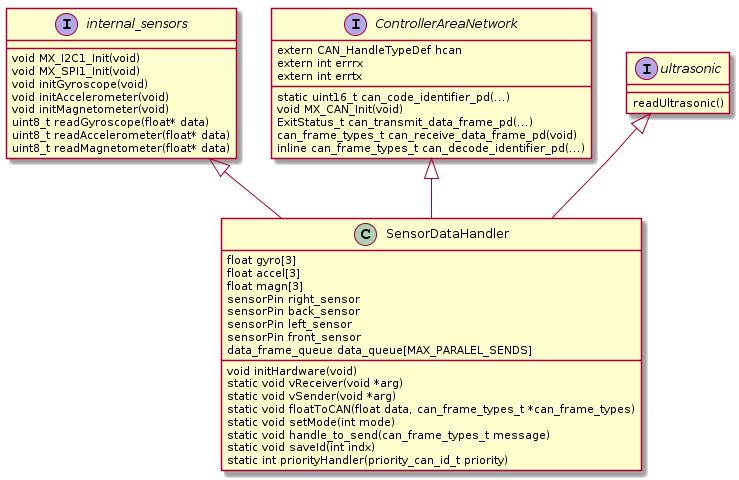
\includegraphics[width=\textwidth]{class}
    \caption{Overview of sources implementation}
    \label{fig:class}
\end{figure}

This code starts to run as soon as the main class calls for the initHardware() function which starts the first FreeRTOS task dedicated to poll for an incoming CAN frame every 10ms. As long as there is no incoming CAN frame the status of the CAN reception will be timeout. When a CAN frame is received the status changes for that cycle to ok which starts the logic of the reception part. This logic is as follows: Upon successful reception of a CAN frame, the c\_s\_bit is checked to see if the CAN frame needs a sensor data. If this is the case, the mode of the transmission will be set. The mode is read from the first data byte of the CAN frame and can be:

\begin{itemize}
\item '0' for no transmission. This mode stops the transmission of the requested sensor.
\item '1' for publisher mode. This mode starts a transmitting FreeRTOS task according to the parameters of the second and third data bytes from the CAN frame.
\item '2' for the one time transmission mode. This mode requests only one transmission of a sensor data, regardless and without altering the previous tasks configuration.
\end{itemize}
This modes were set before starting with this project and a brief overview can be inferred by figure \ref{fig:canmodes}
Further explanation of the modes changes and their implementation will be done in the upcoming section.
\begin{figure}[ht]
	\centering
	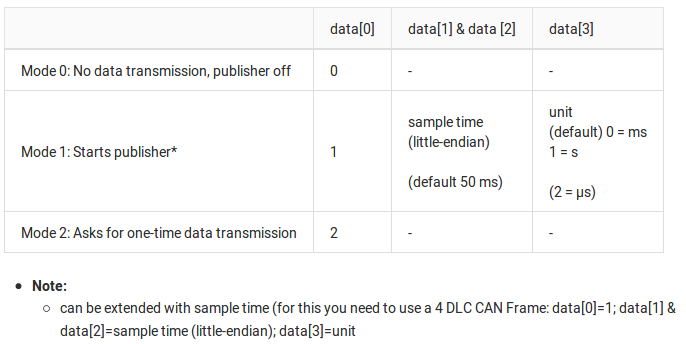
\includegraphics[width=\textwidth]{modes}
    \caption{Modes requested implementation}
    \label{fig:canmodes}
\end{figure}

\section{Implementing Modes}
As discussed before, there are three main modes: no transmission, publisher, and one time transmission. This functionality was implemented with a state machine of those three stages. The behavior can be seen in figure \ref{fig:states}.

The first mode is the no transmission mode. When a CAN frame is received requesting this mode, the CAN frame id is decoded and the topic id of the requested sensor is identified so the FreeRTOS task that was sending its information gets deleted.

The second mode is the publisher mode. In this mode the data from bytes 1 and 2 are decoded taking into consideration figure \ref{fig:canmodes}, which means that the first byte will serve as the time value and the second byte as the requested unit of time. It is important to note that the received data is in bits format which means that the value has to be parsed into an integer first.

Once the time constraint has been set, the next step is to check if the requested sensor is already sending CAN frames with a different frequency. If this is the case, that task will be deleted and replaced with the new one. The FreeRTOS task is then created with the time constraint as a period of time in which the task will be sending data. The rest of the time the task is not sending information, it sleeps itself and wakes up with a relative timer that is set each time the system powers on.

The third mode is the one time transmission mode. In this mode, the requested sensor data will be sent once regardless and without altering the previous tasks configuration.

\begin{figure}[ht]
	\centering
	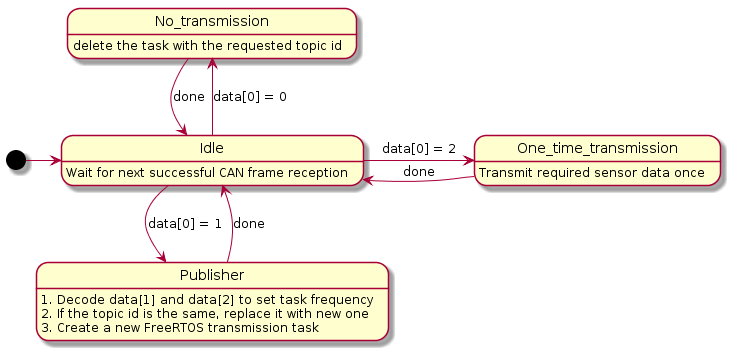
\includegraphics[width=\textwidth]{states}
    \caption{Modes implementation}
    \label{fig:states}
\end{figure}

\section{Real-time implementation}
\label{sect:realtime}
For the real-time implementation certain factors had to come into consideration: the maximum heap size that the FreeRTOS can spare for its tasks, preemption of the tasks so that each task fulfills its deadline, and the priority of each task which contributes to the preemption decision.

Fortunately the preemption of the tasks is done by the FreeRTOS system and the only configuration needed was to turn on the the preemptive functionality and base it on priorities. The priorities of FreeRTOS work backwards as the DAEbot project was establishing. In FreeRTOS the lowest priority is the '0' and it grows accordingly. In the DAEbot project it is established that the highest priority has to be '0' so a normalization had to be done. This job is being done by the function priorityHandler().

The number of possible sending tasks at the same time was set to four. This decision was done with the intention of leaving some free heap of the FreeRTOS maximum heap size configuration for the other sensors and actuators that must be a part of this project and are not ready as of the date of this document: motors and motor encoders. So if there are four sending tasks being executed and the board gets a request for sending a fifth sensor value, this fifth sensor value will not be taken into consideration until one of the previous tasks gets deleted by the user using mode 0.

An example application of the system can be appreciated in figure \ref{fig:timing}, where an example situation is shown.The example was considered as follows:

\begin{enumerate}
\item At 30ms the reception task receives a CAN frame requesting a gyroscope 'x' value every 20ms.
\item At 50ms the reception task receives a CAN frame requesting a accelerometer 'z' value every 10ms.
\item At 70ms the reception task receives a CAN frame requesting a ultrasonic sensor \#2 value one time.
\item At 90ms the reception task receives a CAN frame requesting the ultrasonic sensor \#1 value every 10ms.
\item At 110ms the reception task receives a CAN frame requesting the gyroscope 'x' value to stop being transmitted.
\item At 150ms the reception task receives a CAN frame requesting the magnetometer 'y' value every 30ms.
\item At 170ms the reception task receives a CAN frame requesting the ultrasonic sensor \#3 value every 10ms.
\item At 210ms the reception task receives a CAN frame requesting the ultrasonic sensor \#1 value to stop being transmitted.
\end{enumerate}


\begin{figure}[ht]
	\centering
	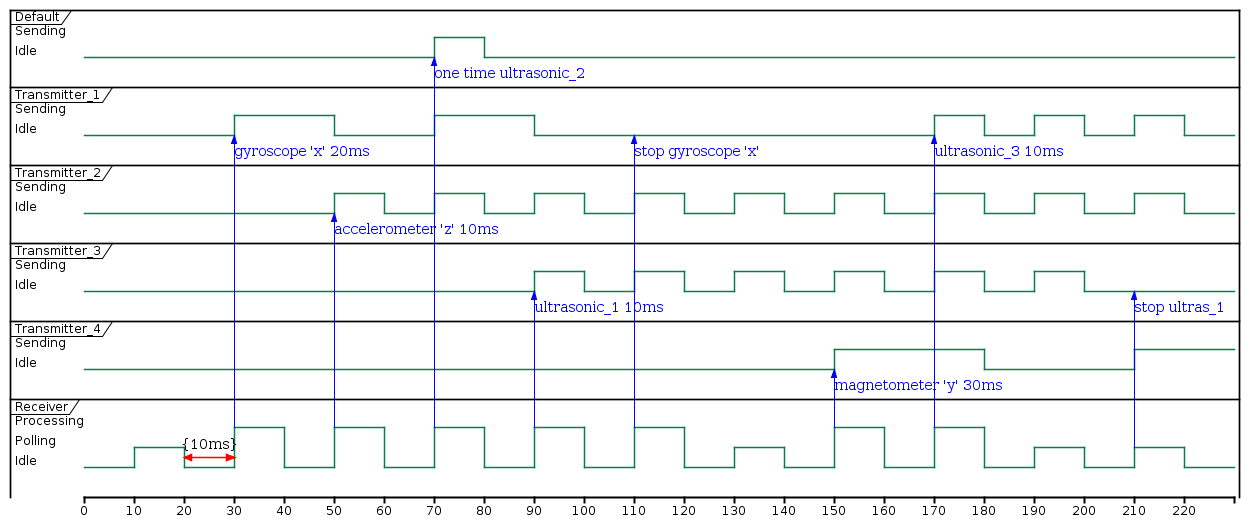
\includegraphics[ width=18cm, height = 10cm, angle = 90]{timing}
  	\caption{Example requests}
  	\label{fig:timing}
\end{figure}

\chapter{Results}
The project was successfully compiled and flashed into the STM32F3 DISCOVERY board. For testing, a CAN-USB interface was used to monitor the CAN low and high signals. The testing case was similar to the one shown in section \ref{sect:realtime}. This test is shown in figures \ref{fig:res2} and \ref{fig:res1}. In \ref{fig:res2} the different CAN frames to be sent are shown. It is important to note that the protocol for the CAN frames to be sent is being followed according to figure \ref{fig:canmodes}. The next process was followed:

\begin{figure}[ht]
	\centering
	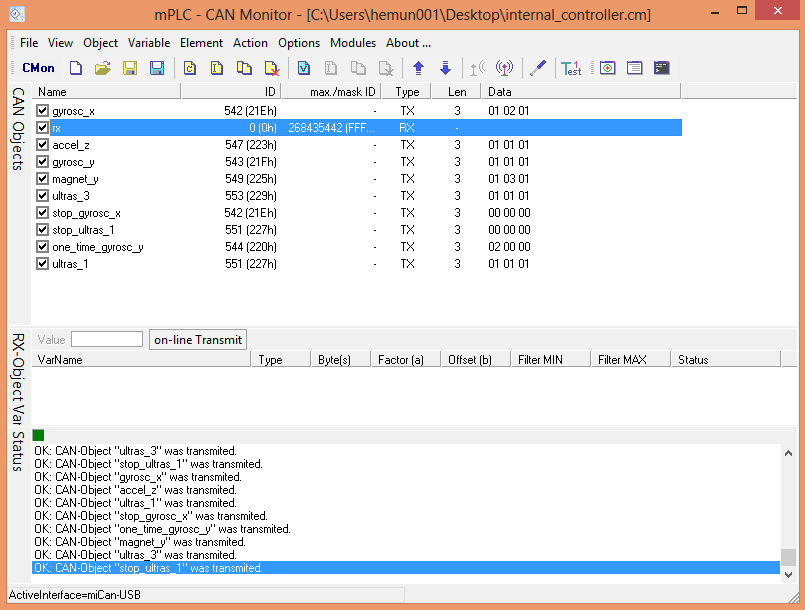
\includegraphics[width=\textwidth]{results_2}
    \caption{CANalyzer configuration.}
    \label{fig:res2}
\end{figure}

\begin{enumerate}
\item The board receives a request for sending gyroscope 'x' (ID equal to 0x21E) values every two seconds.
\item The board receives a request for sending accelerometer 'z' (ID equal to 0x223) values every second.
\item The board receives a request for sending ultrasonic sensor \#1 (ID equal to 0x227) values every second.
\item The board receives a request for stopping sending gyroscope 'x' (ID equal to 0x21E) values.
\item The board receives a request for sending a one time gyroscope 'z' (ID equal to 0x220) value.
\item The board receives a request for sending magnetometer 'y' (ID equal to 0x225) values every three seconds.
\item The board receives a request for sending ultrasonic sensor \#3 (ID equal to 0x229) values every second.
\item The board receives a request for stopping sending ultrasonic sensor \#1 (ID equal to 0x227) values.
\end{enumerate}

Note that the ID's are given by setting the c/s bit to sensor data according to figure \ref{fig:can}, but also using the ID assigned to each sensor according to the Wiki\cite{DAEbot_Wiki}. Also note that the STM32F3DISCOVERY board receives a 0x2'xx' where xx represent the topic id but the '2' indicates that a command is being requested with normal priority, i.e. '010'. The sensor data is then sent with the same topic id but with a '6' instead which means that the CAN frame represents a sensor data with normal priority, i.e. '110'.

\begin{figure}[ht]
	\caption{CAN results}
	\centering
	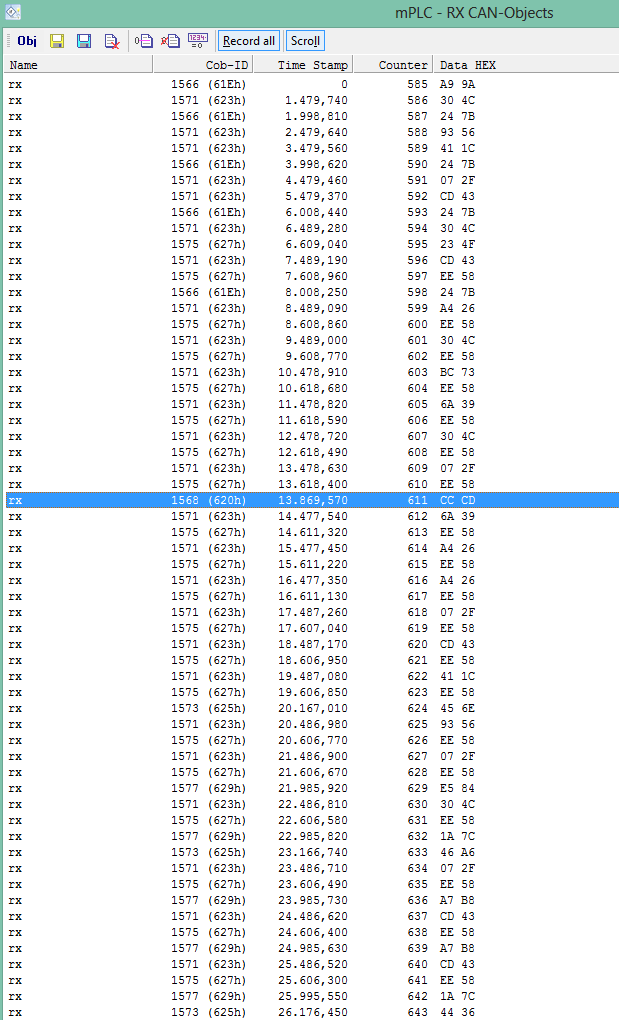
\includegraphics[ width=\textwidth, height = \textheight]{results}
  \label{fig:res1}
\end{figure}

The results are shown in figure \ref{fig:res1}. The average error was of +/-100ns. There were also few bigger errors, the maximum error registered was about 10ms. It is important to mention that these 'big' errors occurred right when there was a reception of a new CAN frame asking for a new sensor data. When there is no new request, the error remains within +/-100ns.

Considering the previous results, it can be said that the overall system is capable of the following:

\begin{enumerate}
\item Access the gyroscope, accelerometer, and magnetometer sensors, as well as the four ultrasonic sensors and obtain the data mapped to real values.
\item Send and receive CAN frames.
\item Use the protocol established in the requirements of the DAEbot with respect of the CAN frames, which means that the frames are coded and decoded according to the protocol.
\item Handling of the received CAN frames and being able to separate between the required modes, no transmission, publisher, and one time transmission.
\item Use a real-time operating system to manage the required scheduler which manages to fulfill the deadlines with a high accuracy.
\end{enumerate}

\section{Outlook}
The project has certain parts where the implementation can be improved in terms of robustness and scalability of number of parallel tasks. For one, the project uses a polling system with the FreeRTOS system, this means that the overall system is parallelized but it is paying a little cost of waiting for timeouts in the reception task, which even thought are small, i.e 100ns - 1ms can result in a loss of accuracy when expecting a result in under this time constraint.

It can be said that the real-time system is working as expected: meeting deadlines and not loosing packages. The error range for this purposes discussed in the previous section is still small enough to make the project fulfill the requirements of a soft real-time system.

As a possible future work the reception and sending of the CAN frames can be done with interruptions so that even less time is consumed in context switching. This would improve both, the capability of maximum number of tasks as well as the robustness of the system. This however, has to be done once the motors and encoders project for the Internal Controller is finished so that these constraints can be modified and tested in the full extension of the STM32F3DISCOVERY board.

Also there is a possibility of selecting a different clock source in order to make the system go from the fixed 8MHz as the input clock, to 32MHz which can be later scaled by the PLL multiplier. This can be achieved by soldering the corresponding pins directly from the board according to the section 6.10.1 from the STM32F3DISCOVERY User Manual\cite{mcu}.
\fi

%bibliography
\printbibliography
\nocite{*}

\end{document}
\grid
